\documentclass[tikz,border=7pt]{standalone}
\usepackage{libertinus}
\usepackage{amsmath}
\usetikzlibrary{
  arrows.meta,
  backgrounds,
  calc,
  decorations.markings,
  fit,
  positioning
}

\definecolor{accent}{RGB}{38,103,115}
\definecolor{softgray}{RGB}{244,245,246}
\definecolor{midgray}{RGB}{123,128,132}

\tikzset{
  >={Latex[length=2.2mm,width=1.5mm]},
  flow/.style={-Latex,semithick,draw=black!72},
  accent flow/.style={-Latex,semithick,draw=accent},
  box/.style={
    draw=black!68,
    fill=softgray,
    rounded corners=1.2pt,
    align=center,
    inner xsep=5pt,
    inner ysep=4pt
  },
  accent box/.style={
    draw=accent,
    fill=accent!8,
    rounded corners=1.2pt,
    align=center,
    inner xsep=5pt,
    inner ysep=4pt
  },
  point/.style={circle,draw=black!75,fill=white,inner sep=1.7pt},
  accent point/.style={circle,draw=accent,fill=accent!10,inner sep=1.7pt},
  tinylabel/.style={font=\scriptsize,align=center},
  smalllabel/.style={font=\small,align=center},
  panel/.style={draw=black!28,rounded corners=2pt,inner sep=6pt}
}


\newcommand{\ordernode}[5][]{%
  \node[box,minimum width=1.12cm,minimum height=.76cm,#1] (#2) at (#3) {#4\\[-2pt]\scriptsize #5};%
}

\begin{document}
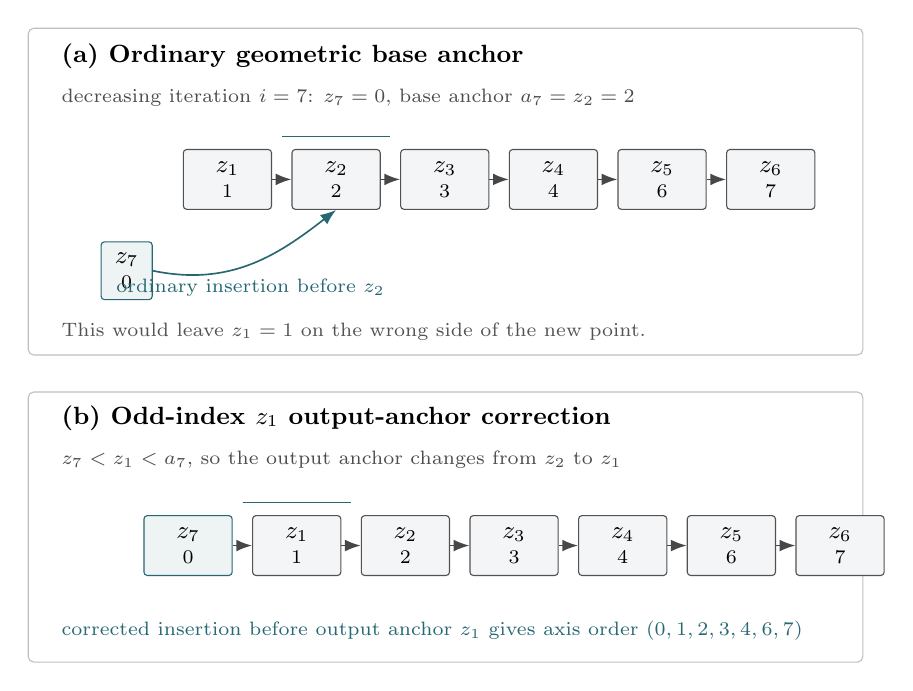
\begin{tikzpicture}[font=\small,x=1cm,y=1cm]
  \node[font=\small\bfseries,anchor=west] at (.15,3.75)
    {(a) Ordinary geometric base anchor};
  \node[font=\scriptsize,anchor=west,text=black!70] at (.15,3.22)
    {decreasing iteration $i=7$: $z_7=0$, base anchor $a_7=z_2=2$};

  \foreach \label/\value [count=\i] in {z_1/1,z_2/2,z_3/3,z_4/4,z_5/6,z_6/7} {
    \ordernode{a\i}{1.0+1.38*\i,2.18}{$\label$}{$\value$}
    \ifnum\i>1
      \draw[flow] (a\the\numexpr\i-1\relax.east) -- (a\i.west);
    \fi
  }
  \node[accent box] (new) at (1.10,1.02) {$z_7$\\[-2pt]\scriptsize $0$};
  \draw[accent flow] (new.east) .. controls (2.4,.82) and (3.0,1.20) ..
    node[below=2pt,font=\scriptsize,text=accent] {ordinary insertion before $z_2$} (a2.south);
  \draw[accent,semithick] ($(a2.north west)+(-.12,.16)$) -- ($(a2.north east)+(.12,.16)$);
  \node[font=\scriptsize,text=black!68,anchor=west] at (.15,.25)
    {This would leave $z_1=1$ on the wrong side of the new point.};

  \node[font=\small\bfseries,anchor=west] at (.15,-.85)
    {(b) Odd-index $z_1$ output-anchor correction};
  \node[font=\scriptsize,anchor=west,text=black!70] at (.15,-1.38)
    {$z_7 < z_1 < a_7$, so the output anchor changes from $z_2$ to $z_1$};

  \foreach \label/\value [count=\i] in {z_7/0,z_1/1,z_2/2,z_3/3,z_4/4,z_5/6,z_6/7} {
    \ifnum\i=1
      \ordernode[draw=accent,fill=accent!8]{b\i}{.50+1.38*\i,-2.47}{$\label$}{$\value$}
    \else
      \ordernode{b\i}{.50+1.38*\i,-2.47}{$\label$}{$\value$}
    \fi
    \ifnum\i>1
      \draw[flow] (b\the\numexpr\i-1\relax.east) -- (b\i.west);
    \fi
  }
  \draw[accent,semithick] ($(b2.north west)+(-.12,.16)$) -- ($(b2.north east)+(.12,.16)$);
  \node[font=\scriptsize,text=accent,anchor=west] at (.15,-3.55)
    {corrected insertion before output anchor $z_1$ gives axis order $(0,1,2,3,4,6,7)$};

  \begin{scope}[on background layer]
    \draw[black!25,rounded corners=2pt] (-.15,-.05) rectangle (10.45,4.10);
    \draw[black!25,rounded corners=2pt] (-.15,-3.95) rectangle (10.45,-.52);
  \end{scope}
\end{tikzpicture}
\end{document}
